%% Adapted from GaTech CS 7545 Machine Learning Theory given by Prof. Jacob Abernathy Fall 2018. Original latex file: https://github.com/mltheory/CS7545/blob/master/scribe/CS7545scribe_template.tex 



%%%%%PLEASE CONSIDER CORRECTIONS AT PLACES INDICATED%%%%%%%%
\documentclass{article}
%%%%%Packages Used, add more if necessary%%%%
\usepackage{amsmath,amsfonts,amssymb,graphicx,fullpage, float}
\setlength{\topmargin}{-0.6 in}
\setlength{\textheight}{8.5 in}
\setlength{\headsep}{0.75 in}
\usepackage{mdframed}
\usepackage{multicol}
\usepackage{microtype}
\usepackage{hyperref}


%%%%% NO NEED TO EDIT THIS PREAMBLE %%%%%%%%
%%% PREAMBLE %%%
\newcounter{lecnum}
\renewcommand{\thepage}{\thelecnum-\arabic{page}}
\renewcommand{\thesection}{\thelecnum.\arabic{section}}
\renewcommand{\theequation}{\thelecnum.\arabic{equation}}
\renewcommand{\thefigure}{\thelecnum.\arabic{figure}}
\renewcommand{\thetable}{\thelecnum.\arabic{table}}
\newcommand{\lecture}[4]{
   \pagestyle{myheadings}
   \thispagestyle{plain}
   \newpage
   \setcounter{lecnum}{#1}
   \setcounter{page}{1}
   \noindent
   \begin{center}
   \framebox{
      \vbox{\vspace{2mm}
      
      \hbox to 6.28in { 
      {\bf ECE 4252/6252 (FunML) Fundamentals of Machine Learning \hfill 2021--2028} }
      
      \vspace{2mm}
      \hbox to 6.28in { 
      {Courses developed by Professor Ghassan AlRegib 
      (\href{https://alregib.ece.gatech.edu/}{alregib.ece.gatech.edu}) 
      \hfill For inquiries: \href{mailto:alregib@gatech.edu}{alregib@gatech.edu}} }
      
      \vspace{3mm}
      \hbox to 6.28in { {\Large \hfill Lecture #1: #2 \hfill} }
      
      \vspace{2mm}
      \hbox to 6.28in { {\it Co-Instructors: #3 \hfill #4} }
      
      \vspace{2mm}}
   }
   \end{center}

   % -------- PEOPLE OUTSIDE BOX --------
   \vspace{2mm}
   \noindent{\bf Contributors:} Dr. Ahmad Mustafa, Dr. Motaz Alfarraj, Dr. Ashraf Alattar, Dr. Chen Zhou

   \vspace{1mm}
   \noindent{\bf Teaching Assistants} with remarkable contributions include: Kuo-Wei Lai, Wuyang Du, Shiva Mahato, Michael Zhou, Ninghan Zhong

   \markboth{Lecture #1: #2}{Lecture #1: #2}

   \vspace{2mm}
\noindent {\bf Disclaimer}: 
{All content of these notes are part of this course at Georgia Tech. Any re-use or distribution is not permitted without pre-approved permission. All these notes belong to, created by, and copyrighted for Ghassan AlRegib and Mohit Prabhushankar, Georgia Tech, 2021--2028.}

\vspace{2mm}
\noindent {\bf License}: 
{These lecture notes are licensed under the 
\href{https://creativecommons.org/licenses/by-nc-sa/4.0/}{Creative Commons Attribution-NonCommercial-ShareAlike 4.0 International License}.}

   \vspace{2mm}
   \noindent {\bf Errata}: 
   {\it Please submit any errata you find using the following form: 
   \href{https://forms.office.com/r/fbg9dMWPgY}{Errata Form for FunML Textbook} 
   or visit: \url{https://forms.office.com/r/fbg9dMWPgY}}

   \vspace*{4mm}
}
\renewcommand{\cite}[1]{[#1]}
\def\beginrefs{\begin{list}
        {[\arabic{equation}]}{\usecounter{equation}
         \setlength{\leftmargin}{2.0truecm}\setlength{\labelsep}{0.4truecm}%
         \setlength{\labelwidth}{1.6truecm}}}
\def\endrefs{\end{list}}
\def\bibentry#1{\item[\hbox{[#1]}]}

\newcommand{\challenge}[2]{\noindent \textbf{(Challenge Problem)} \emph{#1}: #2 }

\newcommand{\exercise}[1]{\noindent \textbf{(Exercise)} #1 }

\newcommand{\fig}[3]{
			\vspace{#2}
			\begin{center}
			Figure \thelecnum.#1:~#3
			\end{center}
	}
%%% END_OF_PREAMBLE %%%


	
%%%%You may add more \newtheorem if necessary%%%%%%
\newtheorem{theorem}{Theorem}[lecnum]
\newtheorem{lemma}[theorem]{Lemma}
\newtheorem{proposition}[theorem]{Proposition}
\newtheorem{claim}[theorem]{Claim}
\newtheorem{corollary}[theorem]{Corollary}
\newtheorem{definition}[theorem]{Definition}
\newenvironment{proof}{{\bf Proof:}}{\hfill\rule{2mm}{2mm}}


\newcommand{\dom}{\mathrm{dom}}
\begin{document}

\lecture{12}{Gaussian Mixture Models and Image Segmentation}{Ghassan AlRegib and Mohit Prabhushankar}{}%

\noindent\textbf{Keywords:} Gaussian mixture models, expectation-maximization, clustering, unsupervised learning, representation learning

\section{Lecture Objectives}

In the previous lecture we introduced k-means clustering as a hard-clustering method. In this lecture, we extend clustering to a probabilistic setting by introducing \textbf{Gaussian Mixture Models (GMMs)}, which perform \textbf{soft clustering}. We study how GMM parameters are estimated using the \textbf{Expectation--Maximization (EM)} algorithm. Finally, we explore \textbf{image segmentation as a clustering problem}, including feature representations, color spaces, and clustering-based segmentation methods.

% \section{Lecture Objectives}

% In the previous lecture we introduced k-means clustering and its variants as \textbf{hard-clustering} methods. In this lecture, we extend clustering to a probabilistic setting by introducing \textbf{Gaussian Mixture Models (GMMs)}, which perform \textbf{soft clustering} by modeling data as a mixture of multivariate Gaussians and inferring posterior responsibilities. We then study how GMM parameters are estimated using the \textbf{Expectation--Maximization (EM)} algorithm (and why EM is needed in latent-variable models compared to direct MLE), and we evaluate clustering quality using both \textbf{internal} metrics (e.g., Davies--Bouldin, Dunn, Silhouette) and \textbf{external} metrics (e.g., Rand Index, Mutual Information, Purity) when ground truth is available. Finally, we study \textbf{image segmentation as a clustering problem}, where pixels are grouped into meaningful regions using clustering algorithms such as k-means, GMMs, and mean shift. We also discuss how segmentation performance is evaluated using specialized metrics.

% \section{Recap From Last Lecture} 
% k-means and its variant are all hard-clustering methods. Thereby those methods fail to works very successfully when:

% %%%%%Use itemize to layout bullet points that are not numbered%%%%%
% \begin{itemize}
% \item Clusters are not near symmetrical in shape (distance to cluster centroid is different)
% \item Overlap exists between clusters

% \end{itemize}
% Therefore, the Clustering method, \textbf{Gaussian Mixture Model}, a probabilistic model for representing several \textbf{normally distributed} data within an overall \textbf{data distribution}, is needed to deal with situations k-means clustering can't handle well.

\section{GMM Clustering}

\subsection{Definition of GMM Clustering}
Assume the data $x_1,x_2,...x_N \in \mathbb{R}^{p}$ are random variables drawn independent and identically from an unknown distribution with probabilistic density $Q(x)$. GMM estimates the likelihood of $Q(x)$ with a \textbf{linear superposition} of $k$ \textbf{multivariate Gaussian distributions} can be denoted by:\[
Q(x) = \sum_{j=1}^{k}\pi_{j}q_{j}(x)=\sum_{j=1}^{k}\pi_{j}\mathcal{N}   (x|\mu_{j},\Sigma_{j})
\]
Where $\mathcal{N}(x|\mu_{j}\Sigma_{j})$ is the \textbf{Gaussian Distribution} denoted by:\[
\mathcal{N}(x|\mu_{j}\Sigma_{j})=\frac{1}{(2\pi)^{\frac{p}{2}}|\Sigma|^{\frac{1}{2}}}e^{-\frac{1}{2}(x-\mu_{j})^{T}\Sigma_{j}^{-1}(x-\mu_{j})}
\]
in which, the parameters\\
$\mu = \{\mu_1,...\mu_k\}, \: \mu_{j} \in \mathbb{R}^{p}$ is the \textbf{cluster means};\\
$\Sigma = \{\Sigma_1,...,\Sigma_k\}, \: \Sigma_{j} \in \mathbb{R}^{p\times p}$ is the \textbf{cluster covariance matrices} (Multi-variant equivalent of standard deviation);\\
$\pi = \{\pi_1,...,\pi_k\}, \: \pi_{j}\in \mathbb{R}$ is the \textbf{cluster coefficients} (Multi-variant equivalent of prior/likelihood) selecting $\mathcal{N}(x|\mu_{j}\Sigma_{j})$, satisfying $\sum_{j=1}^k \pi_j = 1$\\
% Note:
% \begin{itemize}
%     \item GMM is a \textbf{Generative model} which specifically model $p(z_i = j)$ and $p(X_i|z_i = j)$
%     \item GMM is a \textbf{soft clustering method}, which computes the probability of sach sample generated from each cluster.
%     \item Given a sufficiently large number of mixture components, a GMM can be used to approximate \textbf{any density} defined on $\mathbb{R}^p$
%     \item GMM can be though of using Naive Bayes calculation of probability with the assignment algorithm of k-means
% \end{itemize}

\paragraph{GMM as a generative model.}
A Gaussian Mixture Model (GMM) is a \emph{generative} model: it describes a probabilistic mechanism by which the observed data are produced. Concretely, it introduces a latent (unobserved) cluster indicator variable $z_i \in \{1,\dots,k\}$ for each sample $x_i$. The model specifies (i) a prior distribution over components, $p(z_i=j)=\pi_j$ with $\pi_j \ge 0$ and $\sum_{j=1}^k \pi_j = 1$, and (ii) a class-conditional distribution for the data given the component, $p(x_i \mid z_i=j)=\mathcal{N}(x_i \mid \mu_j, \Sigma_j)$. Marginalizing out the latent variable $z_i$ yields the mixture density $Q(x)=\sum_{j=1}^k \pi_j \mathcal{N}(x \mid \mu_j, \Sigma_j)$ \cite{2}.

\paragraph{Soft clustering interpretation.}
Unlike hard clustering methods (e.g., k-means) that assign each point to exactly one cluster, GMMs provide a \emph{soft} assignment. For each sample $x_i$, the model computes a posterior probability of belonging to each component,
$\gamma_i^j = p(z_i=j \mid x_i)$, often called the \emph{responsibility} of component $j$ for explaining $x_i$. These responsibilities quantify uncertainty: if $x_i$ lies in an overlap region between clusters, then multiple $\gamma_i^j$ values may be non-negligible. In practice, one may still obtain a hard label by taking $\arg\max_j \gamma_i^j$, but the probabilistic assignments contain richer information than a single label.

\paragraph{Approximating arbitrary densities.}
GMMs are flexible density estimators. Intuitively, each Gaussian component can model a “local” region of the distribution, and the weighted sum of many such components can represent complex, multimodal, and non-spherical shapes. With a sufficiently large number of mixture components (and appropriate parameters), mixtures of Gaussians can approximate a wide class of smooth probability densities on $\mathbb{R}^p$ to arbitrary accuracy. This is one reason GMMs are widely used as a general-purpose probabilistic model for clustering and density estimation \cite{2}.

\paragraph{Connection to Naive Bayes and k-means.}
A helpful way to view GMM clustering is as combining ideas from probabilistic classification and centroid-based assignment. The posterior responsibility $\gamma_i^j$ follows directly from Bayes’ rule, similar in spirit to a Naive Bayes classifier: it compares how likely $x_i$ is under each component, weighted by the prior $\pi_j$, and then normalizes across $j$. At the same time, the iterative EM updates resemble k-means: in the E-step, points are “assigned” (softly) to components via responsibilities; in the M-step, the component parameters are updated using these assignments (with responsibilities acting as weights). In the special case where all covariances are equal and spherical, the EM procedure recovers behavior closely related to k-means, but the full GMM allows elliptical clusters and overlapping components.

\subsection{Estimation with GMM Clustering}
Similar as other methods, we could also implement MLE estimation for GMM clustering, and write the likelihood function and log likelihood function as follows:\[
L(x,\pi,\mu,\Sigma)=\prod_{i=1}^{N}Q(x_i)=\prod_{i=1}^{N}\sum_{j=1}^{k}\pi_{j}\mathcal{N}(x|\mu_{j},\Sigma_{j})
\]
\[
LL(x,\pi,\mu,\Sigma)=\sum_{i=1}^{N}log\{\sum_{j=1}^{k}\pi_{j}\mathcal{N}(x|\mu_{j},\Sigma_{j})\}\]
However, since the existence of clustering structure (log of sum), there is \textbf{no close-form maxima} for the likelihood function except for $k=1$ ($\mu_{MLE}=\frac{1}{N}\sum_{i}^{N}x_i$, $\Sigma_{MLE}=\frac{1}{N}\sum_{i=1}^{N}(x_i-\mu_{MLE})(x_i-\mu_{MLE})^{T}$).\\
Therefore, we could utilize the \textbf{Expectation Maximization (EM) Algorithm} \cite{1}, which iteratively estimates the mean $\mu_j$ with $\gamma_i^{j}$, and in turn estimates the posterior.\\
The posterior $\gamma_i^{j}$, which is also known as the \textbf{responsibility} of cluster j for sample $x_i$, can be derived using Bayes Rule:\[
\gamma_i^{j}=p(z_i=j|x_i)=\frac{\pi_j\mathcal{N}(x_i|\mu_j,\Sigma_j)}{\sum_{j=1}^{k}\pi_j\mathcal{N}(x_i|\mu_j,\Sigma_j)}
\]\\
The specific steps are as following:
\begin{enumerate}
    \item \textbf{Initialization}: Initialize the mean $\mu_j^{(0)}$, covariance $\Sigma_j^{(0)}$ and mixing coefficient $\pi_j^{(0)}$.\\ (A good initialization is $\mu_j^{(0)} = $random sample $x_i$; $\Sigma_j^(t)=$sample covariance; $\pi_j^{(0)}=\frac{1}{k}$)
    \item \textbf{Expectation}: compute the responsibility with current parameters\[
    (\gamma_i^j)^{(t)}=\frac{\pi_j^{(t)}\mathcal{N}(x_i|\mu_j^{(t)},\Sigma_j^{(t)})}{\sum_{j=1}^{k}\pi_j^{(t)}\mathcal{N}(x_i|\mu_j^{(t)},\Sigma_j^{(t)})}
    \]
    \item \textbf{Maximization}: Re-estimate the parameters using the current responsibilities\[
    \mu_j^{(t+1)}=\frac{\sum_{i=1}^{N}(\gamma_i^{j})^{(t)}x_i}{\sum_{i=1}^{N}(\gamma_{i}^{j})^{(t)}}
    \]
    \[
    \Sigma_j^{(t+1)}=\frac{\sum_{i=1}^{N}(\gamma_i^{j})^{(t)}(x_i-\mu_j^{(t+1)})(x_i-\mu_j^{(t+1)})^{T}}{\sum_{i=1}^{N}(\gamma_i^{j})^{(t)}}
    \]
    \[
    \pi_j^{(t+1)}=\frac{1}{N}\sum_{i=1}^{N}(\gamma_i^{j})^{(t)}
    \]
    \item \textbf{Convergence Check}: Evaluate the log likelihood\[
    LL(x,\pi,\mu,\Sigma)=\sum_{i=1}^{N}log\{\sum_{j=1}^{k}\pi_{j}\mathcal{N}(x|\mu_{j},\Sigma_{j})\}
    \] to see if there's convergence, given by\[
    |(LL(x,\pi,\mu,\Sigma))^{(t+1)} - (LL(x,\pi,\mu,\Sigma))^{(t)}| \leq \epsilon
    \]if not, go back to step 2.
\end{enumerate}

% \subsection{Aside: EM vs MLE}
% It's important to appreciate the difference between the introduced EM approach above and MLE which we've seen before. In MLE, we optimize the likelihood of parameters directly by finding the values that maximize the likelihood function. However, in more complex cases where there are hidden (\textbf{latent}) variables, a direct MLE (or even MAP) estimate may not be possible. In these cases, we invoke EM as an iterative approximation of the MLE/MAP estimates. Note that EM is a general optimization technique that extends beyond GMM. In general, it consists of the two main steps:
% \begin{itemize}
%     \item \textbf{Expectation (E-Step):} Compute the expected value of the log-likelihood function, with respect to the current distribution of the latent variables (the responsibilities in the case of GMM). This step effectively ``fills in" the latent information by computing a distribution over the latents.
%     \item \textbf{Maximization (M-Step):} Maximize this expected log-likelihood with respect to the model parameters. This step refines the parameter estimates based on the expectations from the E-Step.
% \end{itemize}

\subsection{Aside: EM vs MLE}

It is important to distinguish between Maximum Likelihood Estimation (MLE) and the Expectation–Maximization (EM) algorithm introduced above \cite{1,2}. In classical MLE, we directly maximize the likelihood function with respect to the model parameters. This is feasible when the likelihood has a tractable analytical form or when gradients can be computed directly. However, in many realistic models—including Gaussian Mixture Models—there exist hidden (\textbf{latent}) variables that are not observed in the data. The presence of these latent variables makes the likelihood involve a logarithm of a sum, which prevents a closed-form maximization and makes direct MLE (or even MAP estimation) difficult.

The EM algorithm provides an iterative strategy for obtaining MLE or MAP estimates in such latent-variable models. Rather than optimizing the incomplete-data likelihood directly, EM alternates between estimating the missing latent information and optimizing the parameters given those estimates. Importantly, EM is a general optimization framework and is not limited to GMMs; it is widely used in many probabilistic models that involve hidden variables.

In the \textbf{Expectation step (E-step)}, the algorithm computes the expected value of the complete-data log-likelihood with respect to the current distribution of the latent variables. Intuitively, this step “fills in’’ the missing information by estimating how likely each latent configuration is under the current parameter values. In the case of GMMs, this corresponds to computing the responsibilities $\gamma_i^j$, which represent the probability that each data point was generated by each mixture component.

In the \textbf{Maximization step (M-step)}, the algorithm updates the model parameters by maximizing this expected log-likelihood. Using the responsibilities as soft assignments, the parameters are re-estimated to better explain the data. The E-step and M-step are repeated until the log-likelihood converges, guaranteeing a monotonic increase in the likelihood at each iteration.

\subsection{Example of GMM Clustering}
We are going to implement EM Algorithm for a Gaussian mixture of 2 models.
\subsubsection{Initialization}
We can initialize the EM Algorithm as follows:
\begin{figure}[H]
    \centering
    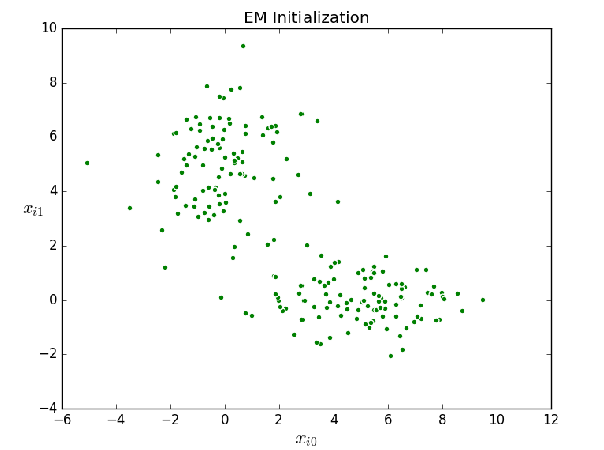
\includegraphics[width=0.4\linewidth]{img/lecture12/GMM clustering Examples/Initialization of EM algorithm.png}
    \caption{Figure 12.1: Initialization of EM Algorithm}
\end{figure}
\subsubsection{Iteration 0}

We can calculate the parameters for iteration $0^{th}$ as following:\\
Cluster Means:
\[
\mu_1 = 
\begin{bmatrix}
0.6496 \\
4.6208
\end{bmatrix}, \quad
\mu_2 = 
\begin{bmatrix}
4.7642 \\
0.2020
\end{bmatrix}
\]

Cluster Covariances:
\[
\Sigma_1 = 
\begin{bmatrix}
5.3102 & 0.0000 \\
0.0000 & 4.2118
\end{bmatrix}, \quad
\Sigma_2 = 
\begin{bmatrix}
5.4851 & 0.0000 \\
0.0000 & 1.7956
\end{bmatrix}
\]
Cluster Means:
\[
\mu_1 = 
\begin{bmatrix}
1.1000 \\
2.1000
\end{bmatrix}, \quad
\mu_2 = 
\begin{bmatrix}
2.9000 \\
3.9000
\end{bmatrix}
\]

Cluster Covariances:
\[
\Sigma_1 = 
\begin{bmatrix}
1.1052 & 0.0000 \\
0.0000 & 2.2103
\end{bmatrix}, \quad
\Sigma_2 = 
\begin{bmatrix}
3.3155 & 0.0000 \\
0.0000 & 4.4207
\end{bmatrix}
\]
\begin{figure}[H]
    \centering
    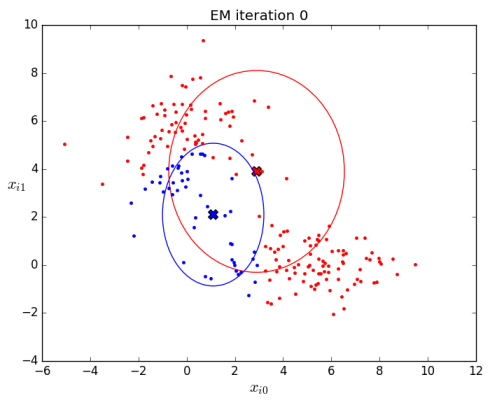
\includegraphics[width=0.4\linewidth]{img/lecture12/GMM clustering Examples/Iteration 0 of EM algorithm.png}
    \caption{Figure 12.2: Iteration 0 of EM Algorithm}
\end{figure}

\subsubsection{Iteration 50}
We can calculate the new parameters for iteration $50^{th}$ as following:\\

Cluster Means:
\[
\mu_1 = 
\begin{bmatrix}
2.0690 \\
3.0228
\end{bmatrix}, \quad
\mu_2 = 
\begin{bmatrix}
2.7500 \\
2.2505
\end{bmatrix}
\]

Cluster Covariances:
\[
\Sigma_1 = 
\begin{bmatrix}
5.5456 & 0.0000 \\
0.0000 & 7.5187
\end{bmatrix}, \quad
\Sigma_2 = 
\begin{bmatrix}
9.9789 & 0.0000 \\
0.0000 & 7.4052
\end{bmatrix}
\]
\begin{figure}[H]
    \centering
    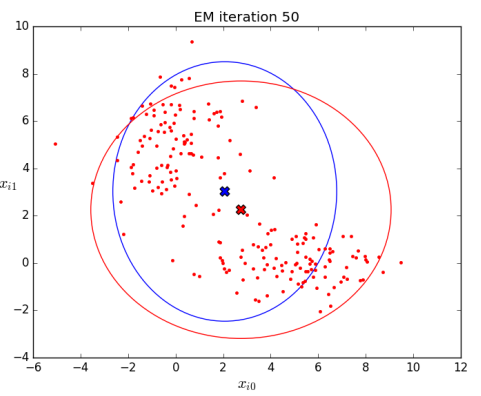
\includegraphics[width=0.4\linewidth]{img/lecture12/GMM clustering Examples/Iteration 50 of EM Algorithm.png}
    \caption{Figure 12.3: Iteration 50 of EM Algorithm}
\end{figure}

\subsubsection{Iteration 100}
We can calculate the parameters for iteration $100^{th}$ as following:\\

Cluster Means:
\[
\mu_1 = 
\begin{bmatrix}
0.6496 \\
4.6208
\end{bmatrix}, \quad
\mu_2 = 
\begin{bmatrix}
4.7642 \\
0.2020
\end{bmatrix}
\]

Cluster Covariances:
\[
\Sigma_1 = 
\begin{bmatrix}
5.3102 & 0.0000 \\
0.0000 & 4.2118
\end{bmatrix}, \quad
\Sigma_2 = 
\begin{bmatrix}
5.4851 & 0.0000 \\
0.0000 & 1.7956
\end{bmatrix}
\]
\begin{figure}[H]
    \centering
    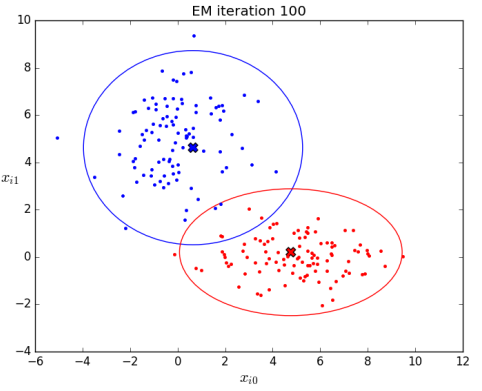
\includegraphics[width=0.4\linewidth]{img/lecture12/GMM clustering Examples/Iteration 100 of EM Algorithm.png}
    \caption{Figure 12.4: Iteration 100 of EM Algorithm}
\end{figure}

\subsubsection{Iteration 150}
We can calculate the parameters for the $150^{th}$ iteration as following:\\

Cluster Means:
\[
\mu_1 = 
\begin{bmatrix}
0.6496 \\
4.6208
\end{bmatrix}, \quad
\mu_2 = 
\begin{bmatrix}
4.7642 \\
0.2020
\end{bmatrix}
\]

Cluster Covariances:
\[
\Sigma_1 = 
\begin{bmatrix}
5.3102 & 0.0000 \\
0.0000 & 4.2118
\end{bmatrix}, \quad
\Sigma_2 = 
\begin{bmatrix}
5.4851 & 0.0000 \\
0.0000 & 1.7956
\end{bmatrix}
\]
\begin{figure}[H]
    \centering
    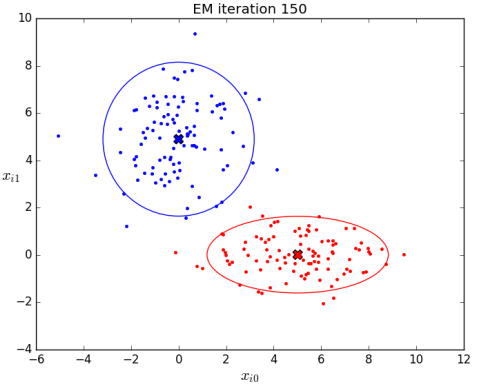
\includegraphics[width=0.4\linewidth]{img/lecture12/GMM clustering Examples/Iteration 150 of EM Algorithm.png}
    \caption{Figure 12.5: Iteration 150 of EM Algorithm}
\end{figure}

Keep iterating until the log likelihood converges. Note:
\begin{itemize}
    \item The diagonals of the cluster covariances are standard deviations and measure the length of the cluster shape on an axis.
\end{itemize}

While Gaussian Mixture Models provide a flexible probabilistic framework for clustering, it is equally important to understand how clustering methods are applied in real-world settings. One particularly important application is image segmentation, where clustering is used to group pixels into meaningful regions based on similarity.

% ============================================================
% NEW SECTION STARTS HERE
% ============================================================
\section{Image Segmentation as a Clustering Problem}

Clustering methods such as k-means, Gaussian Mixture Models (GMMs), and mean shift can be applied to real-world data such as images. One important application is \textbf{image segmentation}, where the goal is to partition an image into meaningful regions.

\subsection{Images as Feature Representations}

An image consists of a grid of pixels. Each pixel can be represented as a feature vector. In the simplest case:

\[
x_i = [R_i, G_i, B_i]
\]

Segmentation can therefore be formulated as a clustering problem where each pixel is assigned to a cluster based on similarity.

% % ---------------- FIGURE 1 ----------------
% \begin{figure}[H]
% \centering
% 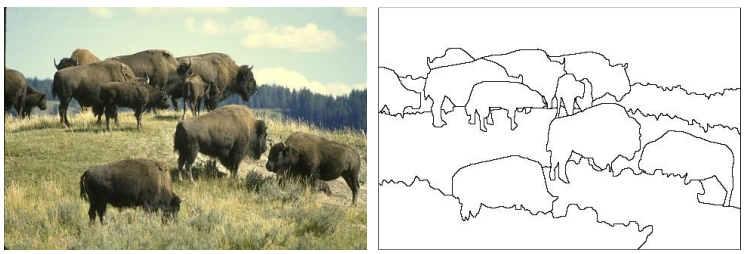
\includegraphics[width=0.6\textwidth]{img/lecture12/segmentation_example.png}
% \caption{Example of image segmentation where pixels are grouped into clusters based on color similarity.}
% \end{figure}

\subsection{Color Spaces for Segmentation}

RGB space is not ideal for clustering because it does not align well with human perception. Alternative color spaces such as LAB are often preferred in image segmentation pipelines because they separate luminance and chrominance more effectively \cite{4}:

\[
x_i = [L_i, a_i, b_i]
\]

This makes clustering more meaningful.

\begin{figure}[H]
\centering

\begin{minipage}[t]{0.16\textwidth}
    \centering
    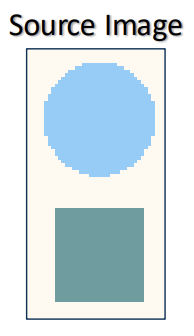
\includegraphics[width=\linewidth]{img/lecture12/source_image.png}
    \vspace{2pt}
    
    \textbf{Source Image}
\end{minipage}
\hspace{0.02\textwidth}
\begin{minipage}[t]{0.133\textwidth}
    \centering
    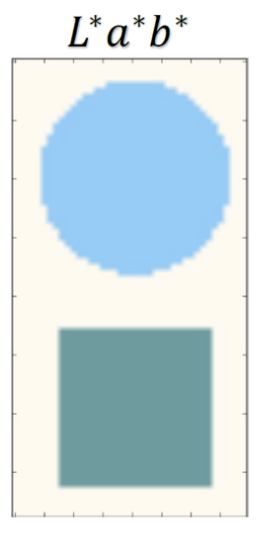
\includegraphics[width=\linewidth]{img/lecture12/gmm.png}
    \vspace{2pt}
    
    \textbf{GMM ($L^*a^*b^*$)}
\end{minipage}

\caption{Effect of color space on clustering-based segmentation. The source image is shown on the left, while GMM segmentation in the $L^*a^*b^*$ color space is shown on the right.}
\end{figure}

\subsection{Feature Construction for Pixels}

Pixel features can include spatial information:

\[
x_i = [L_i, a_i, b_i, x_i, y_i]
\]

This encourages spatially close pixels to belong to the same segment.

\subsection{Clustering-Based Segmentation Methods}

\begin{itemize}
    \item \textbf{k-means}: a hard-clustering method that assigns each pixel to exactly one cluster. It is efficient, but requires specifying the number of clusters $k$ in advance.
    \item \textbf{GMM}: a soft-clustering method that assigns pixels according to posterior probabilities, making it more flexible when color distributions overlap.
    \item \textbf{Mean Shift}: a density-based method that finds clusters as modes of the feature distribution and does not require specifying the number of clusters beforehand \cite{3}.
\end{itemize}

We now compare how different clustering algorithms produce segmentation results on the same image:

\begin{figure}[H]
\centering

\begin{minipage}[t]{0.181\textwidth}
    \centering
    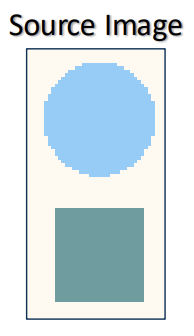
\includegraphics[width=\linewidth]{img/lecture12/source_image.png}
    \vspace{2pt}
    
    \textbf{Source}
\end{minipage}
\hspace{0.02\textwidth}
\begin{minipage}[t]{0.15\textwidth}
    \centering
    
\includegraphics[width=\linewidth]{img/lecture12/kmeans.png}
    \vspace{2pt}
    
    \textbf{k-means}
\end{minipage}
\hspace{0.02\textwidth}
\begin{minipage}[t]{0.15\textwidth}
    \centering
    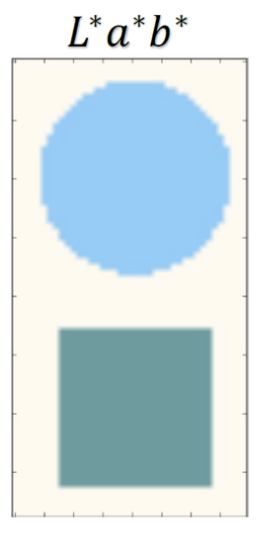
\includegraphics[width=\linewidth]{img/lecture12/gmm.png}
    \vspace{2pt}
    
    \textbf{GMM}
\end{minipage}
\hspace{0.02\textwidth}
\begin{minipage}[t]{0.15\textwidth}
    \centering
    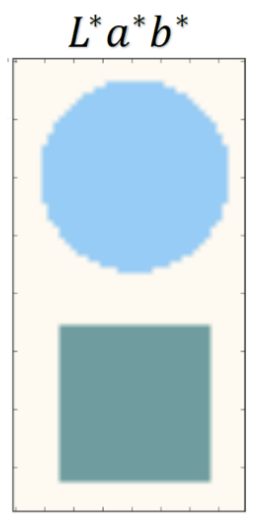
\includegraphics[width=\linewidth]{img/lecture12/mean_shift.png}
    \vspace{2pt}
    
    \textbf{Mean Shift}
\end{minipage}

\caption{Segmentation results produced by different clustering methods. The original image is shown on the left, followed by segmentations obtained using k-means, GMM, and mean shift. Each method produces slightly different partitions depending on its modeling assumptions.}
\end{figure}


\subsection{Connection to Homework 4}

\textbf{Connection to HW4:} In Homework 4, segmentation is performed by clustering pixels into groups based on their feature representations. The choice of feature space (RGB vs LAB) and clustering method directly affects performance.

\newpage

\section{Q\&A Section}

\begin{enumerate}
    \item \textbf{Question 1:} \newline
    Which statement best describes the difference between \textbf{k-means} and \textbf{GMM} clustering?
    
    \begin{enumerate}
        \item k-means performs soft clustering, while GMM performs hard clustering.
        \item k-means assigns each point to exactly one cluster, while GMM assigns posterior probabilities to clusters.
        \item k-means models each cluster with a full covariance matrix, while GMM uses only centroids.
        \item There is no difference; both methods are equivalent in general.
    \end{enumerate}
    
    \textbf{Solution:} \newline
    The correct answer is \textbf{(b)}. k-means is a \textbf{hard-clustering} method that assigns each sample to exactly one cluster, whereas GMM is a \textbf{soft-clustering} method that computes posterior probabilities (responsibilities) for each cluster.

    \vspace{6pt}

    \item \textbf{Question 2:} \newline
    In the EM algorithm for GMMs, what is computed during the \textbf{E-step}?
    
    \begin{enumerate}
        \item Updated cluster means and covariance matrices
        \item Posterior responsibilities for each data point under each component
        \item The optimal number of clusters
        \item A hard assignment of each point to its nearest centroid
    \end{enumerate}
    
    \textbf{Solution:} \newline
    The correct answer is \textbf{(b)}. In the \textbf{E-step}, the algorithm computes the \textbf{responsibilities}
    \[
    \gamma_i^j = p(z_i=j \mid x_i),
    \]
    which represent the posterior probability that sample $x_i$ was generated by component $j$.

    \vspace{6pt}

    \item \textbf{Question 3:} \newline
    Why is the \textbf{LAB} color space often preferred over \textbf{RGB} for clustering-based image segmentation?
    
    \begin{enumerate}
        \item LAB always reduces the number of segments.
        \item LAB separates luminance and chrominance, making perceptual similarity more meaningful for clustering.
        \item LAB guarantees perfect segmentation.
        \item RGB cannot be used for clustering.
    \end{enumerate}
    
    \textbf{Solution:} \newline
    The correct answer is \textbf{(b)}. LAB is often preferred because it separates \textbf{luminance} from \textbf{chrominance}, which better reflects perceptual similarity and can produce more meaningful clusters for segmentation.
\end{enumerate}

\section{References}

\beginrefs

\bibentry{1} Dempster, A. P., Laird, N. M., \& Rubin, D. B. (1977). \textit{Maximum likelihood from incomplete data via the EM algorithm}. Journal of the Royal Statistical Society: Series B.

\bibentry{2} Bishop, C. M. (2006). \textit{Pattern Recognition and Machine Learning}. Springer.

\bibentry{3} Comaniciu, D., \& Meer, P. (2002). \textit{Mean shift: A robust approach toward feature space analysis}. IEEE Transactions on Pattern Analysis and Machine Intelligence.

\bibentry{4} Achanta, R., Shaji, A., Smith, K., Lucchi, A., Fua, P., \& Süsstrunk, S. (2012). \textit{SLIC superpixels compared to state-of-the-art superpixel methods}. IEEE Transactions on Pattern Analysis and Machine Intelligence.

\endrefs

\end{document}
